\section{Cryptographic Protocols and Out-of-Band Revocation}
\label{sec:crypto}

The security of the Virtual Private Phone rests upon two foundational pillars: strong mutual cryptographic authentication during active sessions, and guaranteed, non-repudiable session revocation when the physical frontend is seized or lost.

\subsection{Mutual Authentication and Handshake Protocol}
To secure the telemetry and streaming channels over hostile networks, the VPP implements a specialized instantiation of the Noise Protocol Framework~\cite{perrin2018noise}, specifically the $\texttt{Noise\_IKpsk2}$ pattern. 

\begin{figure}[h!]
\centering
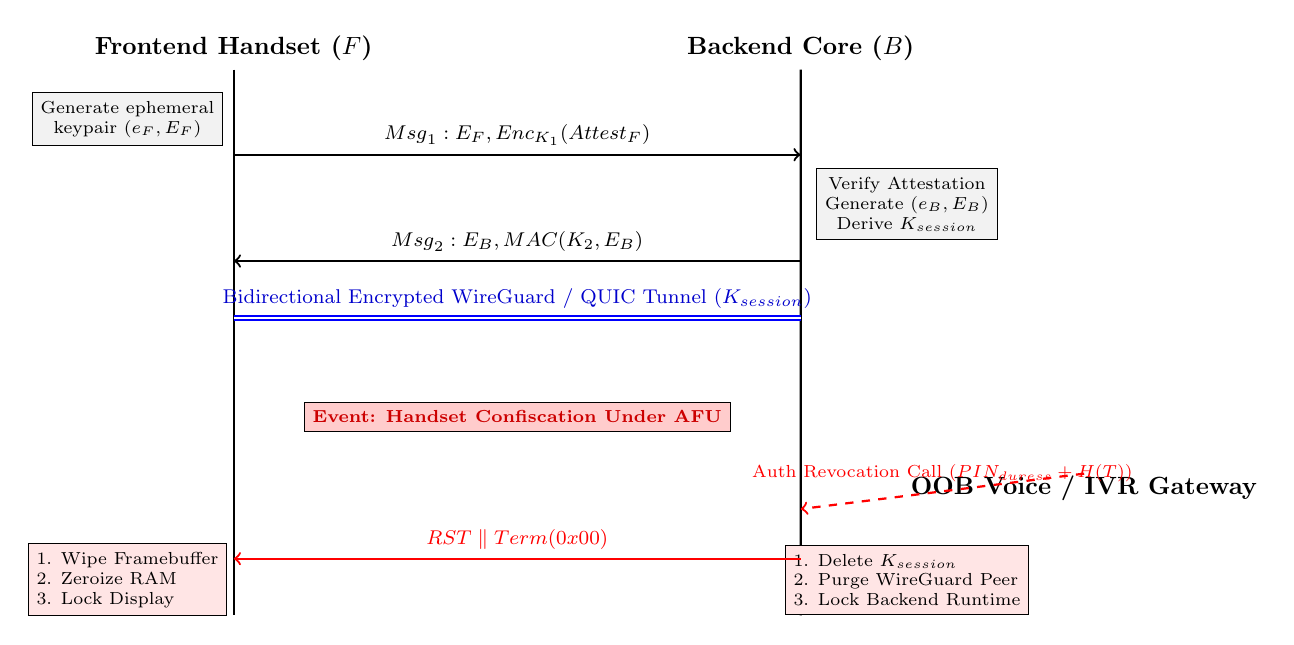
\begin{tikzpicture}[scale=0.9, every node/.style={transform shape}]
    % Actors
    \node (F) at (0, 4) {\textbf{Frontend Handset ($F$)}};
    \node (B) at (8, 4) {\textbf{Backend Core ($B$)}};
    
    \draw[thick] (F) -- (0, -4);
    \draw[thick] (B) -- (8, -4);

    % Step 1: Frontend initiates
    \node[draw, fill=gray!10, font=\scriptsize, align=center] at (-1.5, 3) {Generate ephemeral\\keypair $(e_F, E_F)$};
    \draw[->, thick] (0, 2.5) -- node[above, font=\footnotesize] {$\text{Msg}_1: E_F, \text{Enc}_{K_1}(\text{Attest}_F)$} (8, 2.5);
    
    % Step 2: Backend response
    \node[draw, fill=gray!10, font=\scriptsize, align=center] at (9.5, 1.8) {Verify Attestation\\Generate $(e_B, E_B)$\\Derive $K_{\text{session}}$};
    \draw[<-, thick] (0, 1.0) -- node[above, font=\footnotesize] {$\text{Msg}_2: E_B, \text{MAC}(K_2, E_B)$} (8, 1.0);

    % Established tunnel
    \draw[double, thick, blue] (0, 0.2) -- node[above, font=\footnotesize, text=blue!80!black] {Bidirectional Encrypted WireGuard / QUIC Tunnel ($K_{\text{session}}$)} (8, 0.2);

    % Revocation event
    \node[draw, fill=red!20, font=\scriptsize, text=red!80!black] at (4, -1.2) {\textbf{Event: Handset Confiscation Under AFU}};
    \node (OOB) at (12, -2.2) {\textbf{OOB Voice / IVR Gateway}};
    \draw[->, thick, dashed, red] (12, -2) -- node[above, font=\scriptsize] {Auth Revocation Call ($PIN_{duress} + H(T)$)} (8, -2.5);

    % Cutoff actions
    \node[draw, fill=red!10, font=\scriptsize, align=left] at (9.5, -3.5) {1. Delete $K_{\text{session}}$\\2. Purge WireGuard Peer\\3. Lock Backend Runtime};
    \draw[->, thick, red] (8, -3.2) -- node[above, font=\footnotesize] {$\text{RST} \parallel \text{Term}(0x00)$} (0, -3.2);
    \node[draw, fill=red!10, font=\scriptsize, align=left] at (-1.5, -3.5) {1. Wipe Framebuffer\\2. Zeroize RAM\\3. Lock Display};

\end{tikzpicture}
\caption{Protocol flow for session establishment, remote attestation, and out-of-band revocation.}
\label{fig:protocol_flow}
\end{figure}

The session handshake proceeds as follows:
\begin{enumerate}
    \item \textbf{Identity Keys:} The backend holds a long-term static Curve25519 public key $S_B$. The frontend holds an identity key $S_F$ and pre-configured hardware attestation credentials rooted in its secure hardware.
    \item \textbf{Ephemeral Key Exchange:} The frontend generates an ephemeral keypair $(e_F, E_F)$ and transmits its public component along with an encrypted hardware attestation token confirming that the frontend is running an unmodified $\texttt{dm-verity}$ verified kernel.
    \item \textbf{Session Key Derivation:} Upon verifying the frontend attestation, the backend responds with an ephemeral public key $E_B$. Both parties execute Diffie-Hellman calculations:
    \begin{equation}
        \text{DH}_1 = \text{X25519}(e_F, S_B), \quad \text{DH}_2 = \text{X25519}(e_F, E_B), \quad \text{DH}_3 = \text{X25519}(S_F, E_B)
    \end{equation}
    Symmetric session keys $K_{session} = \langle K_{\text{stream}}, K_{\text{telemetry}} \rangle$ are derived using HKDF-SHA256 with an injected pre-shared key ($PSK$). All subsequent AV1 video frames and touch events are encrypted via ChaCha20-Poly1305 AEAD.
\end{enumerate}

\subsection{The Out-of-Band (OOB) Revocation Protocol}
The defining operational challenge of mobile seizure is that the operator loses physical access to the device at the exact moment revocation is required. An operator in police custody or subject to an armed robbery cannot open the phone's settings menu to execute a self-destruct command.

\subsubsection{1. Emergency Telephone and IVR Gateway}
To resolve this dilemma, the VPP interfaces with an independent, carrier-grade telephony gateway (e.g., automated IVR over Twilio / Telnyx with multi-region redundancy). When the operator is granted a standard phone call (e.g., legal consultation call following arrest) or borrows an unmonitored telephone:
\begin{enumerate}
    \item The operator dials a dedicated 24/7 toll-free emergency number.
    \item The IVR prompts the caller for an operator account identifier ($UID$) and a high-entropy secret emergency passcode ($PIN_{rev}$).
    \item The gateway transmits an authenticated, signed webhook request over an isolated TLS connection directly to the backend listener:
    \begin{equation}
        \sigma_{req} = \text{HMAC-SHA256}(K_{oob}, UID \parallel \text{Timestamp} \parallel \text{Action:Revoke})
    \end{equation}
\end{enumerate}

\subsubsection{2. Backend Enforcement State Machine}
Upon verifying $\sigma_{req}$, the backend core executes the following atomic revocation sequence:
\begin{itemize}
    \item \textbf{Step 1: Cryptographic Severance:} The WireGuard kernel module immediately removes the public key of the active frontend handset:
    \begin{equation}
        \texttt{wg set wg0 peer } S_F \texttt{ remove}
    \end{equation}
    All active UDP connections drop immediately.
    \item \textbf{Step 2: Key Zeroization:} The symmetric session keys $K_{session}$ stored in kernel memory are wiped using $\texttt{explicit\_bzero}$.
    \item \textbf{Step 3: Poison Packet Transmission:} If the frontend is still reachable over the IP network (i.e., not yet placed into a Faraday bag), the backend transmits a signed tear-down token commanding the client to execute an immediate hard reset and memory purge.
    \item \textbf{Step 4: Backend Lockout:} The local display server on the backend immediately terminates the user session, freezing the Android runtime and reverting to a fully encrypted lock screen.
\end{itemize}

\subsection{Client-Side Deterministic Memory Scrubbing}
If the frontend is placed inside a Faraday enclosure prior to the arrival of the poison packet, the client utilizes autonomous watchdog mechanisms to trigger deterministic memory scrubbing.

\subsubsection{Autonomous Heartbeat and Dead-Man Timeout}
The frontend maintains an internal hardware cryptographic timer:
\begin{equation}
    \Delta t_{heartbeat} = t_{current} - t_{last\_packet}
\end{equation}
If $\Delta t_{heartbeat} > \tau_{threshold}$ (configurable between 30 and 120 seconds):
\begin{enumerate}
    \item The video display pipeline immediately clears the hardware framebuffer memory, filling the display controller with static black pixels ($0x00$).
    \item The kernel executes a full cache flush ($\texttt{clean\_and\_invalidate}$) on L1/L2/L3 CPU caches.
    \item All volatile RAM addresses associated with user space execution are overwritten using multi-pass pseudo-random patterns:
    \begin{equation}
        \mathcal{M} \leftarrow 0x00 \quad \Longrightarrow \quad \mathcal{M} \leftarrow 0xFF \quad \Longrightarrow \quad \mathcal{M} \leftarrow \text{PRNG}()
    \end{equation}
    This eliminates any residual electron polarization or capacitance remanence required for cold-boot DRAM extraction~\cite{halderman2008coldboot}.
    \item The device triggers a hardware watchdog reset, returning the handset to a pristine BFU boot state.
\end{enumerate}

\subsection{Formal Proof of Revocation Finality}
\begin{theorem}[Post-Revocation Seclusion]
Let $\mathcal{S}$ denote the state of the backend core. Let $A$ be an adversary in physical possession of the unlocked frontend handset at time $t > t_{rev}$. Under the assumption that the Curve25519 discrete logarithm problem is hard and ChaCha20-Poly1305 is indistinguishable under chosen-ciphertext attack (IND-CCA2), the probability that $A$ can reconstruct any future frame $F_{t+\delta}$ or cause the backend to transition state is negligible:
\begin{equation}
    \mathrm{Adv}_{\mathcal{A}}^{\mathrm{VPP}}(t > t_{rev}) \le \mathrm{negl}(\lambda)
\end{equation}
\end{theorem}

\begin{proof}
Revocation removes $S_F$ from the backend's allowed peer set and destroys $K_{session}$. Any message injected by $A$ through the frontend's physical interface requires re-initiating the Noise handshake. However, re-initiating the handshake requires a valid, registered public key $S_F$ recognized by the backend. Because $S_F$ has been excised from the backend's ACL, all incoming packets from the frontend are discarded at the kernel packet filter ($\texttt{nftables}$ / WireGuard) without decryption or processing. Thus, possession of the physical frontend grants no path back to the backend.
\end{proof}
